% !TEX encoding = UTF-8 Unicode

\documentclass[a4paper]{article}

\usepackage{color}
\usepackage{url}
\usepackage[T2A]{fontenc} % enable Cyrillic fonts
\usepackage[utf8]{inputenc} % make weird characters work
\usepackage{graphicx}
\usepackage{listings}

\usepackage[english,serbian]{babel}

\usepackage[unicode]{hyperref}
\hypersetup{colorlinks,citecolor=green,filecolor=green,linkcolor=blue,urlcolor=blue}

\newtheorem{primer}{Primer}[section]
\newtheorem{definicija}{Definicija}[section]

\begin{document}

\title{Algoritmi za detekciju plagijarizma \\ \small{Seminarski rad u okviru kursa\\Metodologija stručnog i naučnog rada\\ Matematički fakultet}}

\author{Nemanja Subotić, Igor Rodić \\ suboticnemanja93@gmail.com, igorrodic@gmail.com}
\date{9.~april 2016.}
\maketitle

\abstract{
Sa pojavom modernih tehnologija, pre svega interneta, svet je postao u velikoj meri izložen raznim oblicima zloupotreba. Jednu od tih zloupotreba predstavljaju plagijarizmi. Zbog ogromne količine podataka koja je dostupna velikoj većini ljudske civilizacije, lakše je nego ikada naći potrebne informacije o bilo čemu što nas zanima, ali to sa sobom nosi i rizike. Jer skoro sa istom lakoćom bilo ko može te informacije da iskopira (preformuliše, ukrade ideju) i prezentuje kao svoje delo. Prirodno je potražiti odgovor na ovo pitanje u kompjuterskim algoritmima, jer bi taj zadatak za čoveka bio previše obiman. Shodno tome, razvijeni su mnogi algoritmi za detekciju raznih vrsta plagijarizama, koji imaju za cilj automatizovanje procesa otkrivanja plagijata. Njima ćemo se detaljnije baviti u ovom radu.}

\tableofcontents

\newpage

\section{Pomoc}
\label{sec:pomoc} 

Ovde pišem uvodni tekst.
Ovde pišem uvodni tekst. 
Ovde pišem uvodni tekst. 
Ovde pišem uvodni tekst. 

\begin{primer} I tabele treba da budu u svom okruženju, i na njih je neophodno referisati se u tekstu. Na primer, u tabeli \ref{tab:tabela1} su prikazana različita poravnanja u tabelama.

\begin{table}[h!]
\begin{center}
\caption{Razlčita poravnanja u okviru iste tabele ne treba koristiti jer su nepregledna.}
\begin{tabular}{|c|l|r|} \hline
centralno poravnanje& levo poravnanje& desno poravnanje\\ \hline
a &b&c\\ \hline
d &e&f\\ \hline
\end{tabular}
\label{tab:tabela1}
\end{center}
\end{table}

\end{primer}


\section{Uvod}
\label{sec:uvod}

U ovom radu, pored detekcije plagijarizama teksta, bavićemo se i  detekcijom plagijarizama programskog koda, koji je za nas informatičare posebno interesantan.

\section{Ideje i pristupi}
\label{sec:ideje i pristupi}

Prva stvar o kojoj treba diskutovati jeste klasifikacija sistema za detekciju plagijarizama. Ona je, prirodno, za svakoga drugačija. Osnovna podela, prema Mozgovoy-u deli pomenute sisteme na dve podgrupe, na sisteme koji prave "otisak prsta" (eng.~{\em fingerprint}) programa i na sisteme koji porede sadržaj.

%(\ref{fig:klasifikacija}) 
%\begin{figure}[h!]
%\begin{center}
%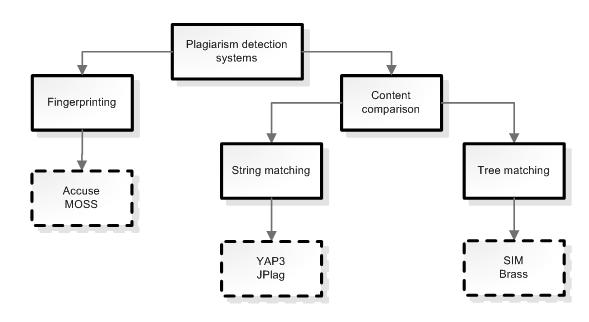
\includegraphics[scale=0.5]{klasifikacija.jpg}
%\end{center}
%\caption{Klasifikacija sistema za detekciju plagijarizama programskog koda}
%\label{fig:klasifikacija}
%\end{figure}

\par "Otiska prsta" programa predstavlja kratku sekvencu bajtova koja karakterizuje duži fajl. On može da se dobije primenom heš (eng.~{\em hash}) funkcije na fajl, ali obično se koristi niz numeričkih atributa (prosečan broj reči po liniji, prosečan broj ključnih reči itd.), i zatim se pomoću funkcije radzdaljine računa stepen različitosti dva fajla. Ova tehnika se danas retko koristi jer čak i male promene mogu da rezultuju potpuno drugačijim "otiscima".
\par Poređenje sadržaja predstavlja osnovu za veliku većinu sistema za detekciju plagijarizama. Ono je generalno zasnovano na Manberovoj definiciji sličnosti i deli se na dve podvrste. One su poredjenje stringova i drveta parsiranja.
\begin{definicija}
Manberova definiciji sličnosti: Kažemo da su dva fajla slična ako sadrže značajan broj istih podniski koje nisu prekratke.
\end{definicija}
Algoritmi za poređenje sadržaja funkcionišu po istom principu:
\begin{lstlisting}
FOR EACH collection file F
  FOR EACH collection file G, F =/= G
    Calculate similarity between F and G
\end{lstlisting}
dok se funkcija za određivanje sličnosti menja. Kada pričamo o poređenju stringova pod time podrazumevamo poređenje fajlova, koji se tretiraju kao veliki stringovi. Logično, ovaj način poređenja ne čuva strukturu fajlova, kao ni programskog koda. Algoritmi koji koriste ovaj način detekcije su: FPDS, koji računa sličnost po formuli:
\begin{lstlisting}
sim(F, G) = MatchedTokens(F, G) / TotalTokens(G)
\end{lstlisting}
YAP (jedan od prvih algoritama ove vrste, koristi poređenje liniju-po-liniju Levenštajnovim rastojanjem), RKR-GST (pravi pokrivač nepreklapajućih stringova koji sadrže maksimalan mogući broj tokena iz oba fajla, algoritam je NP kompletan pa zavisi od uspešnih heuristika, npr. duže podniske su vrednije od kraćih).
Drveta parsiranja sa druge strane očuvavaju strukturu fajla, kako tekstualnog (poglavlja, pasusi itd.) tako i programskog (klase, funkcije itd.). Prednosti ovog metoda poređenja još nisu u potpunosti iskorišćene, jedan od algoritama koji to pokušava je Sim utility. On koristi poređenje stringova, ali ne nad celim fajlovima, već nad njihovim drvetima parsiranja, tj. parser prethodi algoritmu poređenja stringova.

\section{Sakrivanje plagijarizma}
\label{sec:sakrivanje plagijarizma}

\subsection{Tekst}
\label{subsec:tekst}

\subsection{Programski kod}
\label{subsec:programski kod}

Kao što je ranije navedeno, detektovanje plagijarizama programskog koda je oblast koja nas informatičare posebno intrigira. Svako od nas je, u jednom trenutku, svesno ili nesvesno, plagirao tudj kod. Provera plagijarizma programskog koda je nešto što profesori iz oblasti informatike rade svakodnevno, ali još se nije došlo do precizne definicije šta to tačno čini plagijarizam programskog koda. Plagijarizam programskog koda javlja se kada je kod kopiran i/ili izmenjen bez prethodne konsultacije sa autorom. \cite{culwinmacleodlancaster} \newline
\par Definisani su i nivoi modifikacije programskog koda, koji mogu da pomognu bližem razumevanju pojma, tj. da daju uvid u načine na koje plagijarizam programskog koda može da bude sakriven:

\begin{itemize}
\item Izmena komentara
\item Izmena belina
\item Preimenovanje identifikatora
\item Izmena rasporeda blokova koda
\item Izmena rasporeda naredbi unutar blokova
\item Izmena redosleda operatora/operanada u izrazima
\item Izmena tipova podataka
\item Dodavanje redundantnih naredbi ili promenljivih
\item Menjanje naredbi kontrole toka ekvivalentnim naredbama kontrole toka (while u do-while itd.)
\item Menjanje poziva funkcije sa telom funkcije
\end{itemize}

Navedene modifikacije prevazilaze se pretprocesiranjem, konkretno tokenizacijom i parametrizovanim poklapanjem. Tokenizacija pretvara programski kod u niz tokena, time ga spuštajući na gradivni nivo (predstavljajući promenljive, pozive funkcija, naredbe itd.) i eliminišući većinu načina skrivanja. Složenost procesa tokenizacije je linearna, stoga ona ne utiče na kompleksnost finalnog algoritma, medjutim, samim procesom mogu da se izgube važne informacije o sličnostima dva programa. U cilju očuvanja te sličnosti tokenizator se koristi zajedno sa parametrizovanim poklapanjem. Parametrizovano poklapanje smatra dva koda identičnim ako jedan može da se dobije iz drugog primenom konačnog broja zamena identifikatora.

\section{Implementacija algoritma za detekciju plagijarizama tekst}
\label{sec:implementacija algoritma za detekciju plagijarizama tekst}

Stopword n-grams.


\section{Implementacija algoritma za detekciju plagijarizama programskog koda}
\label{sec:implementacija algoritma za detekciju plagijarizama programskog koda}

Diff.

\section{Zaključak}
\label{sec:zakljucak}

Zakljucak. 


\addcontentsline{toc}{section}{Literatura}
\appendix
\bibliography{seminarski} 
\bibliographystyle{plain}

\appendix
\section{Dodatak}

Pored ovog rada, u prilogu se nalaze i izvorni kodovi algoritama koji su implementirani.


\end{document}
